\documentclass[a4paper,12pt]{article}
\usepackage{jheppub}
\usepackage{etoolbox}% http://ctan.org/pkg/etoolbox
    \makeatletter
    \patchcmd{\maketitle}{\@fpheader}{}{}{}
    \makeatother
\usepackage{amsmath}
\usepackage{amsthm}
\usepackage{amsfonts}
\usepackage{amssymb}
\usepackage{hyperref}
\usepackage{textcomp}
\usepackage{listings}
\usepackage{graphicx}% Include figure files
\usepackage{bm}% bold math
\usepackage{color}
\usepackage{verbatim}
%\usepackage{subcaption}

\usepackage{graphicx,color}
\usepackage{epstopdf}
\usepackage{epsfig}
%\usepackage{subfigure}
\sloppy
\usepackage{amsfonts,amsmath,amssymb}


\newcommand{\p}{\partial}
\newcommand{\ph}{\varphi}
\newcommand{\phs}{\phi^*}
\newcommand{\lam}{\lambda}
\newcommand{\la}{\langle}
\newcommand{\ra}{\rangle}
\newcommand{\lr}{\leftrightarrow}
\newcommand{\lar}{\leftarrow}
\newcommand{\rar}{\rightarrow}
\newcommand{\eps}{\epsilon}

\newcommand{\lvec}{\overrightarrow}


\newcommand{\qf}{{\cal Q}_2}
\newcommand{\af}{{\cal A}_2}

\setcounter{tocdepth}{1}


\begin{document}

\title{\textbf{Numerical package for holographic lattices}}
\date{}

% \author{Alexander Krikun}
% \author{}
% \affiliation{ Instituut-Lorentz, Universiteit Leiden, Delta-ITP \\ 
%  \textit{P.O. Box 9506, 2300 RA Leiden, The Netherlands}
% } 

%\abstract{}

%\maketitle

%\newpage
\section{Package Distribution}
There are a number of required packages to run this project, such as numpy, scipy and fft packages. In order to have everyone on the same packages and package versions, the easiest is to use a \emph{virtual environment}, \texttt{virtualenv}. There is more information here \href{https://helpdesk.lorentz.leidenuniv.nl/wiki/doku.php?id=working_with_python}{on the computer documentation wiki}. Below I've given a quick explanation how it would be used
\begin{itemize}
\item Make a directory somewhere on your local machine (not in the project folder) to store the virtual environment and cd into it, like this:
\begin{lstlisting}
$ mkdir python_virtual_env && cd python_virtual_env
\end{lstlisting} This folder is where the packages etc will end up being installed. If you would like to remove the virtual environment, all you have to do is delete the folder it is in. 
\item Now we create the virtual environment. We make a virtualenvironment named \texttt{holo-env} with the command
\begin{lstlisting}
$ virtualenv --python=python3.6 holo-env
\end{lstlisting}
You will see that a directory \texttt{holo-env} has been created in the folder. By default, the only packages that are installed are those that are required to install other packages.
\item To start using the virtualenv, you should run the following: 
\begin{lstlisting}
$ source holo-env/bin/activate
\end{lstlisting}
You will that at it will say \texttt{(holo-env)} at the start of your next line in the terminal. This means that you are now in the virtual environment. Python is then simply run with 
\begin{lstlisting}
$ python infile.py
\end{lstlisting}
You can see the packages that are installed with 
\begin{lstlisting}
$ pip list
\end{lstlisting}
\item Now you can install any package that you like. The packages required to run the project are in the root folder of the project in \texttt{requirements.txt}. You can install the packages in there using 
\begin{lstlisting}
$ pip install -r requirements.txt
\end{lstlisting}
If you want to add a package to the requirements, you should install it in your virtual environment and export the requirement using 
\begin{lstlisting}
$ pip freeze > requirements.txt
\end{lstlisting}
That is really all there is to it. To exit the virtual environment, simply type 
\begin{lstlisting}
$ deactivate
\end{lstlisting}
and you will see that your command line returns to normal.
\end{itemize}
\section{Introduction}
\section{Design of the package}
The package consists of separate modules as shown on Diagram \ref{structure}. It consists of a set of initialization blocks, which include importing the form of equations from Mathematica (or elsewhere), setting up the grid and choosing the initial solution and the parameters of the problem; and the internal loop, where the solution is found after several iterations. For performance purposes it is important to optimize the internal loop, while the initialization blocks only need to preserve the precision of data.

Update 17 April:
The current structure is as follows. The problem is defined by a set of equations (EoMs, coefficients, etc), the input parameters (dimensions, grid spacings, etc). Currently, this is being handled by:
\begin{itemize}
\item Load in the ini file into a setup class. The base setup class has all relevant information to execute a simple nonlinear solve where we just have a set of dynamical fields and constants. In the holo\_setup module you'll see
the Setup class, this is the base class. The easiest way to handle fermions on top of a fixed background is by extending the base class. This is also done in the holo\_setup file, and the only things
it needs extra are the ability to read background data and a modification in terms of the variables that are used.
\item The main solver routine is now in a class, NonlinearSolver, which has the main method "solve". This is the main routine: it evaluates derivatives, makes the
updates, etc. Preconditioning using a lower-order approximation of the operator has also been implemented. 
convergence, there are callbacks available to do additional processing (e.g. smoothing, checkpointing, enforcing constraints) to aid in the evaluation process. There is also
the convergence hook, which naturally checks for convergence etc. I have still to implement a working version of it, but it should not take much time. I have included an example of a
'timed hook', which could for example be used to checkpoint the run every so often.
\item Fermions. Fermions I have put in a different section of code because it is so different. It requires its own setup, it requires its own file-reading utilities etc. It is working properly now though, and we should be able to use it. The main ingredients missing are what we actually want from the fermions, e.g. how we wish to calculate Green's functions etcetera. 
\end{itemize}

\begin{figure}[ht]
\center
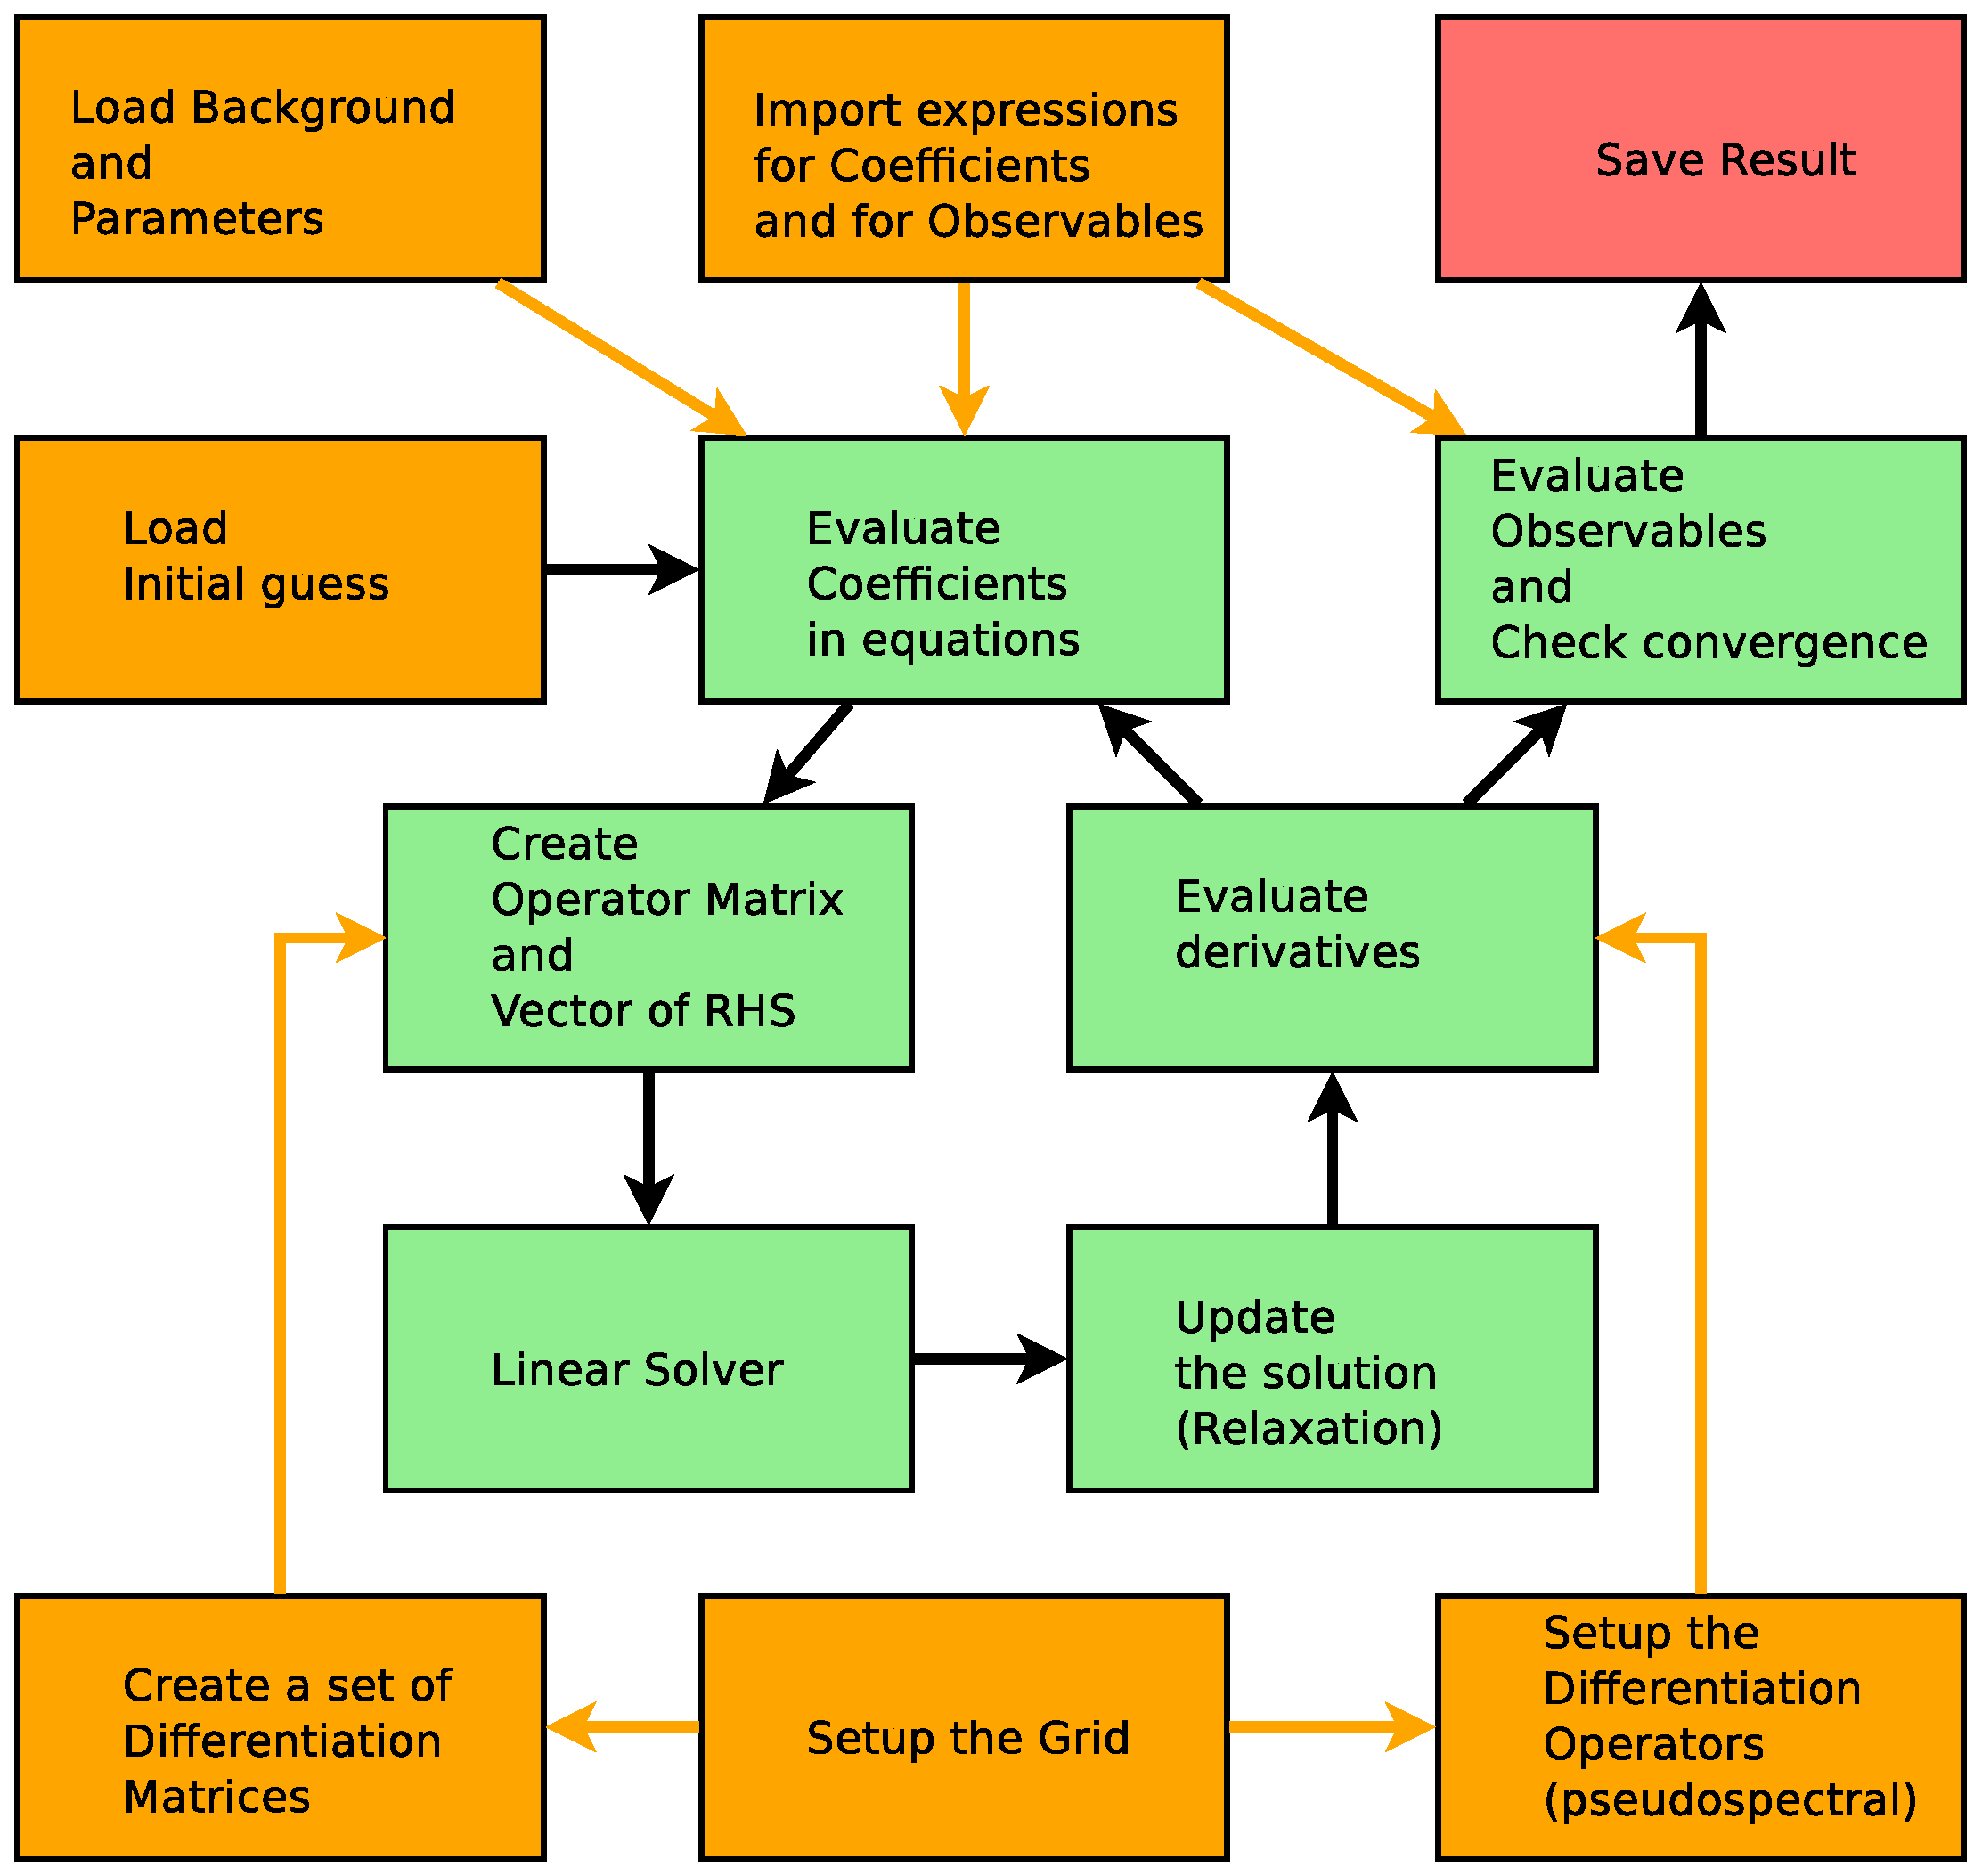
\includegraphics[width=0.8 \linewidth]{Package_Structure.eps}
\caption{\label{structure} \textbf{Principal structure of the package.} Yellow blocks -- initialization, Green blocks -- parts of the loop, which deserve optimization. Arrows show the flow of data. The data structures are explained in the text.}
\end{figure}

\section{Initialization blocks}

\subsection{\label{sec:io_data} Input/Output of data}
This is relevant to the blocks \textbf{Load Background and Parameters}, \textbf{Load Initial Seed} and \textbf{Save Result}. The data should be organized in a unified way as discussed in \ref{sec:file_name}


\subsection{\label{sec:import_expressions}Import expressions for Coefficients and for Observables}
This is a block which converts data from Mathematica to Python. It works together with the Mathematica counterpart, which prepares the arrays of coefficients in the appropriate way.

\subsection{\label{sec:setup_grid} Setup the Grid}
This block should create the appropriate grids, taking as input the number of points in each direction, type of the grid (either \textbf{Homogeneous} or \textbf{Pseudospectral}) and type of the boundary conditions (either \textbf{periodic} or not).

\subsection{\label{sec:diff_mat}Create a set of Differentiation matrices}
It takes the gridpoints and the creates the ``next neighbour'' order diff matrices for a set of derivatives. The outcome is organized as an array with matrices, which include in various dimensions 3, 6 or 10 of them
\begin{align}
\label{order_of_derivatives}
\mbox{1D}: & \qquad \{ \mathbf{1}, \mathbb{D}_{x}, \mathbb{D}_{x x} \} \\
\mbox{2D}: & \qquad \{ \mathbf{1}, \mathbb{D}_{x}, \mathbb{D}_{y}, \mathbb{D}_{xx}, \mathbb{D}_{yy}, \mathbb{D}_{xy} \} \\
\mbox{3D}: & \qquad \{ \mathbf{1}, \mathbb{D}_{x}, \mathbb{D}_{y},\mathbb{D}_{z}, \mathbb{D}_{xx}, \mathbb{D}_{yy}, \mathbb{D}_{zz}, \mathbb{D}_{xy}, \mathbb{D}_{xz}, \mathbb{D}_{yz} \}
\end{align}
The subtlety here is that the grid may not be homogeneous. In practice we need matrices only for homogeneous and Chebyshev lattices, with either periodic or not boundary conditions.

\subsection{\label{sec:diff_oper} Setup the Differentiation Operators}
This block prepares the operator which will be used in order to evaluate derivatives with high precision. This is either a set of Fourier transforms for pseudospectral case or high order differentiation matrices for FDD case. It return the set of operators in the same order as \eqref{order_of_derivatives}

\section{Loop blocks}

\subsection{\label{sec:eval_coefs} Evaluate Coefficients in equations}
This get the expressions for the coordinate dependent coefficients and the values of function and its derivatives on the grid. The latter is organized as a set of $d$-dimensional arrays, which represent the function itself, and its derivatives in order of \eqref{order_of_derivatives} on the $d$-dimensional grid. For instance in 2D  this is
\begin{equation}
\label{fatF}
\mathbb{F} = \{F_{ij}, (\p_x F)_{ij}, (\p_y F)_{ij}, (\p_{xx} F)_{ij}, (\p_{yy} F)_{ij}, (\p_{xy} F)_{ij} \}
\end{equation}
This block makes as many evaluations as there are grid points at every step. It might deserve optimization through compilation of the coefficient functions, maybe even in C.

It returns the coefficients as arrays of the shape $\{ ne, nf * nd, nx , ny, \dots$, where $ne$ is the number of equations, $nf * nd$ -- the number of different terms in the equation, i.e. $nd$ possible derivatives of $nf$ possible functions. 

\subsection{\label{sec:construct_oper} Create Operator Matrix and Vector of RHS}
This one multiplies the evaluated coefficients by the appropriate differentiation matrices and sums over, creating an BVP operator. It also takes care of implementing the boundary conditions in the right way. 

It will also create the vector of right hand sides, which just consists of appropriate nonhomogeneous coefficients evaluated in the previous block.

This one requires clever working with sparse matrices

\subsection{\label{sec:linear_sol} Linear Solver}
As simple as it is. 

\subsection{\label{update_sol} Update the solution}
It updates the solution according to the specified rule. For instance for relaxation
\begin{equation}
F_{i+1} = F_{i} - \frac{3}{7} df
\end{equation}

\subsection{\label{sec:eval_deriv} Evaluate derivatives}
Evaluated the derivatives using the Differential operators defined at Initialization step. Returns the data structure of \eqref{fatF}

\subsection{\label{sec:eval_observables} Evaluate observables and Check convergence}
Checks convergence according to the specified rule and stops the cycle.

\begin{table}[ht]

\center

\begin{tabular}{|l|l|l|}
\hline
\textbf{Input} & \textbf{Block} & \textbf{Output} \\
\hline
\hline
Data file name \ref{sec:file_name} & \textbf{Load Background} \ref{sec:io_data}  & Solution on the grid \ref{sec:solution_data} \\[0.1 cm]
&  & Parameters \ref{sec:params}\\[0.1 cm]
\hline
Data file name \ref{sec:file_name} & \textbf{Load Initial Seed} \ref{sec:io_data} & Solution on the grid \ref{sec:solution_data}  \\[0.1 cm]
\hline
Solution on the grid \ref{sec:solution_data}  & \textbf{Save Result} \ref{sec:io_data} &  Data file name \ref{sec:file_name} \\[0.1 cm]
Parameters \ref{sec:params} & &  \\
Observables \ref{sec:observable_set} & &  \\[0.1 cm]
\hline
Files with coefficients \ref{sec:coef_files} & \textbf{Import Coefficients} \ref{sec:import_expressions} & Evaluator of coefficients \ref{sec:evaluator_coef} \\[0.1 cm]
\hline
Files with observables \ref{sec:observ_files} & \textbf{Import Observables} \ref{sec:import_expressions} & Evaluator of observables \ref{sec:evaluator_coef} \\[0.1 cm]
\hline
Grid parameters \ref{sec:grid_params}& \textbf{Setup the grid} \ref{sec:setup_grid} & Coordindate arrays \ref{sec:coord_arrays} \\[0.1 cm]
\hline 
Grid parameters \ref{sec:grid_params} & \textbf{Create Diff.Matrices} \ref{sec:diff_mat} & Set of Diff. Matrices \ref{sec:diff_mat_set} \\
 Coordindate arrays \ref{sec:coord_arrays} & & \\[0.1 cm]
 \hline
Grid parameters \ref{sec:grid_params} & \textbf{Create Diff.Operators} \ref{sec:diff_oper} & Set of Diff. Operators \ref{sec:diff_oper_set} \\[0.1 cm]
\hline
\hline
Evaluator of coefficients \ref{sec:evaluator_coef} & \textbf{Evaluate coefficients} \ref{sec:eval_coefs} & Set of coefficients \ref{sec:set_coef} \\
Parameters \ref{sec:params} & & \\
Grid parameters \ref{sec:grid_params} & & \\
Coordindate arrays \ref{sec:coord_arrays}  & & \\
Solution with derivatives \ref{sec:solution_deriv_data} & & \\[0.1 cm] 
\hline
Set of coefficients \ref{sec:set_coef} & \textbf{Create operator and RHS} \ref{sec:construct_oper} & Operator and RHS \ref{sec:BVP_oper} \\
Set of Diff. Matrices \ref{sec:diff_mat_set} & & \\[0.1 cm] 
\hline
Operator and RHS \ref{sec:BVP_oper} & \textbf{Linear Solver} \ref{sec:linear_sol} & Adjustmets for solution \ref{sec:adjustment_data} \\[0.1 cm] 
\hline
Adjustmets for solution \ref{sec:adjustment_data} & \textbf{Update solution} \ref{update_sol} & Solution on the grid \ref{sec:solution_data} \\[0.1 cm] 
\hline
Solution on the grid \ref{sec:solution_data}  & \textbf{Evaluate derivatives} \ref{sec:eval_deriv} & Solution with derivatives \ref{sec:solution_deriv_data} \\
Set of Diff. Operators \ref{sec:diff_oper_set} & & \\[0.1 cm]
\hline
Evaluator of observables \ref{sec:evaluator_coef} & \textbf{Evaluate observables} \ref{sec:eval_observables} & Observables \ref{sec:observable_set} \\
Solution with derivatives \ref{sec:solution_deriv_data} & & Stop signal \\
Adjustmets for solution \ref{sec:adjustment_data} & & \\[0.1 cm]
\hline






\end{tabular}

\caption{\label{table:data_structure}Input and output data structures of the blocks}

\end{table}


\section{\label{sec:data_structures} Data structures}

\subsection{\label{sec:file_name} Data file names ans structure}
The solutions are saved in the data files. The file contains the array:
\begin{equation}
\{ \mbox{params}, \mbox{observables}, \mbox{solution} \}
\end{equation}
Keeping the information about physical parameters (\ref{sec:params}), observables (\ref{sec:observable_set}) and the solution itself together with coordinate arrays in the form of \ref{sec:solution_data}. 


{}
\subsection{\label{sec:solution_data} Solution on the grid}

The solution on the grid is represented as $\{ne+d, nx, ny, \dots \}$ array, where $ne$ is a number of functions to be solved for, $nx1,\dots$ the sizes of grid in corresponding directions and $d$ is the number of dimensions in the problem, so that the last $nd$ entries on the first level are the values of corresponding coordinates of the grid points

\subsection{\label{sec:adjustment_data} Adjustments of Solution}

The adjustments have similar structure to \ref{sec:solution_data}, but contain only the values for $ne$ functions (without grid coordinates) 
\begin{equation}
df \sim \mathrm{solution}[[1;;ne,All,All]]
\end{equation}

\subsection{\label{sec:solution_deriv_data} Solution with derivatives on the grid}

This structure holds the values of the functions together with their derivatives. It is compatible with the symbols used in the exported coefficient arrays \eqref{equ:gft}. It is the array of the shape:
\begin{equation}
\mathbb{F} \sim \{nf, nD, nx, ny, \dots \},
\end{equation}
Where $nD$ is the order of derivative according  to \eqref{order_of_derivatives}, $nf$-- the number of function in the ansatz and $nx,ny, \dots$ -- coordinates on the grid.


\subsection{\label{sec:params} Parameters} 
These are the physical parameters of the problem, which enter symbolically the equations of motion. For instance temperature, period of the lattice etc. 

For a particular case of striped background the set is:
\begin{equation}
\label{equ:params}
\mbox{params} = \{T,A,k,N_k,N_p,\phi,c_1 \},
\end{equation}
where $T$ is temperature in units of chemical potential $\mu$, $A$ -- the amplitude of the lattice, $k$ -- the wavevector of the lattice in units of $\mu$, $N_k$ -- number of lattice cells in the computational domain, $N_p$ -- number of periods of spontaneous structure in the domain, $\phi$ -- the phase in the background lattice and $c_1$ -- the coefficient in CS term.

\subsection{\label{sec:observable_set} Set of observables}
These may include free energy, charge density ets, evaluated for particular solution. In the same set one can include the control structures, like accuracy or precision of the final solution, validity of constraints or the number of iterations it took to converge.

\subsection{\label{sec:coef_files} Files with coefficients exported from Mathematica}
The coefficients of equations are exported from Mathematica in the file which contains a number of strings. There are $ne*nD*nf$ strings in the coefficient file. These correspond to the flattened array of coefficients of the shape:
\begin{equation}
\label{equ:exp_coef}
\mbox{exported coefficients} \sim \{ne, nD, nf\}
\end{equation}
Where $ne$ is the number of the equation, $nf$ -- the number of functions in the ansatz, $nD$ -- the order of derivative. More details about these coefficients (called $\mathbf{X}$) are in the lecture notes \cite{Krikun:2018ufr}

The lines include the recognizable mathematical functions in FORTRAN style, the symbols for physical parameters \ref{equ:params} and the symbols for background functions and their derivatives. The last one looks like
\begin{equation}
\label{equ:gfi}
\mathtt{f}[nf,nD]
\end{equation}
Where the first index is the number of function in ansatz and the second is the order of derivative according to \eqref{order_of_derivatives}.

There are several files with coefficients, representing the sytem of equations to be solved internally (\texttt{CoefEOMsI}), and on the boundaries.

Similar is the structure of the exported expressions for nonlinear Right Hand Sides, except that in these files there are only $ne$ lines, containing the nonlinear equations in terms of $\mathtt{gfi}$.

\subsection{\label{sec:set_coef} Set of evaluated coefficients}
The coefficients are evaluated on the grid and are first arranged in the array:
\begin{equation}
\label{equ:coef}
\mathtt{coef} \sim \{ne, nD, nf, nx, ny, \dots  \}
\end{equation}
This shape corresoponds to the exported coefficients \eqref{equ:exp_coef}, evaluated on the grid points.
\subsection{Output of the background solver}
Eventually, all IO will be done using the HDF5 file format (see e.g. h5py documentation). In this format, we can directly save and load numpy arrays. Furthermore, it can handle multidimensional arrays very well, and it has a very logical structure. You save data in datasets, which can have other data as attributes. We will save the following parameters: \\
\begin{tabular}{|p{3cm}|p{3.5cm}|p{5cm}|p{3.5cm}|}
\hline
Data & Type &  Location & Attributes \\
\hline \hline
Field Solutions & numpy ndarray& \textbackslash{}field & periodicity, gridTypes, nDims, nFields, nEOM \\
\hline
Deriv Methods for EOM & list of string & \textbackslash{}controls\textbackslash{}EOMDerivMethods & None\\ \hline
constants & dictionary & \textbackslash{}controls\textbackslash{}parameters & None \\ \hline
Final update & numpy ndarray & \textbackslash{}controls\textbackslash{} & None \\ \hline
Observables & Dict of name-ndarray & \textbackslash{}observables\textbackslash{}\ldots & None \\ \hline
Residual of EOM & numpy ndarray & \textbackslash{}EOMResidual & None \\ \hline

\end{tabular}
\subsection{\label{sec:observ_files} Files with observables exported from Mathematica}
These files contain a few lines, each of them corresponds to a certain observable expressed in terms of parameters \eqref{equ:params} and background functions \eqref{equ:gfi}.

\subsection{\label{sec:evaluator_coef} Evaluator of coefficients or observables}
This must be an object, which contains the symbolic expressions for coefficient and is capabel to quickly evaluate the coefficient on the grid in the form \eqref{equ:coef}.

\subsection{\label{sec:grid_params} Parameters of the grid}
Three arrays, storing the number of points in every direction, the type of grid (``homogeneous'' or ``pseudospectral'') and the type of boundary conditions (periodic: ``True'' or ``False''), it might be a good idea to store explicitely the number of dimentions $d$ and the number of eqiations $ne$
\begin{equation}
\label{equ:grid_data}
\mbox{Grid data} \sim
\{d , ne, \{nx, ny, \dots\}, \{(\mathtt{True}| \mathtt{False}), \dots \}, \{(\mathtt{True}| \mathtt{False}), \dots \} \}
\end{equation}

\subsection{\label{sec:coord_arrays} Coordinate arrays}
This is the array with coordinates in every direction
\begin{equation}
\label{equ:coord_arrays}
\mbox{Coord. arrays} \sim
\{\{x_1, x_2 , \dots\}, \{y_1, y_2 , \dots\}, \dots \}
\end{equation}

\subsection{\label{sec:diff_mat_set} Set of Differentiation Matrices}
The array containing differentiation matrices (sparse) in the order defined in \eqref{order_of_derivatives}.

\subsection{\label{sec:BVP_oper} Boundary Value Problem operator and vector of RHS}
BVP operator is a sparse matrix of the size $\{(ne*nx*ny*\dots) \times (ne*nx*ny*\dots)\}$. Vector of RHS is a dense vector of the compatible size.

\subsection{\label{sec:diff_oper_set} Set of Differentiation Operators}
The array containing differentiation operatore in the order defined in \eqref{order_of_derivatives}.


\begin{thebibliography}{100}
%\cite{Krikun:2018ufr}
\bibitem{Krikun:2018ufr} 
  A.~Krikun,
  %``Numerical Solution of the Boundary Value Problems for Partial Differential Equations. Crash course for holographer,''
  arXiv:1801.01483 [hep-th].
  %%CITATION = ARXIV:1801.01483;%%


\end{thebibliography}

\end{document} 